\subsection{Etilene}

L'etilene \`e stato scelto quale composto di riferimento per la descrizione
della superficie di potenziale descritta dai gradi di libert\`a di interesse.
Per descrivere la molecola si \`e fatto uso della base 6-31G*, con un CAS 2/2
comprendente gli orbitali $\pi$ e $\pistar$

\begin{figure}[ht]
\begin{center}
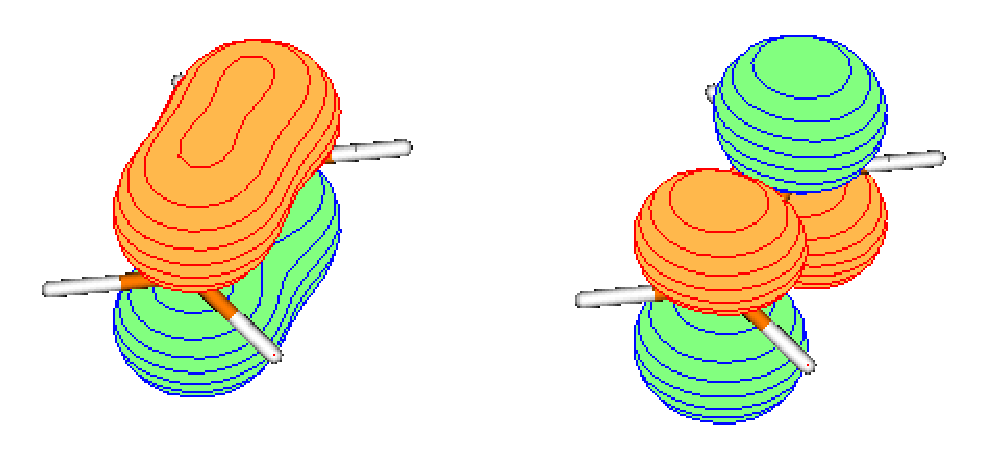
\includegraphics[angle=0,width=7cm,keepaspectratio]{immagini/etene/orbitali.eps}
\parbox[h]{10cm}{
\caption{\small Etilene - orbitali $\pi$ e $\pistar$}
\label{fig:etene_orbitali}
}
\end{center}
\end{figure}

I parametri geometrici in condizioni di equilibrio sono rappresentati in
tabella \ref{tab:etene_geom}, confrontati con un calcolo CASSCF
2/11 con base 6-311(2+)G* (Cfr . \cite{jcp-105-20-1996-9007})
\begin{center}
\begin{threeparttable}
\caption{\small Etilene - geometria per lo stato fondamentale}
\label{tab:etene_geom}
\small
\begin{tabular}{|ccc|c|}
\hline
							& GS		& GS CAS 2/11\tnote{1} \\ 
\hline
$r$(C-C)					& 1.338		& 1.338	\\
$r$(C-H)					& 1.076		& 1.076	 \\
$\angle$(H-C-C)				& 121.7		& 121.7	 \\
\hline
\end{tabular}
\begin{tablenotes}
\small
 \item[1] Cfr. \cite{jcp-105-20-1996-9007}
\end{tablenotes}
\end{threeparttable}
\end{center}

Facendo riferimento alla disposizione degli atomi data in figura
\begin{figure}[ht]
\begin{center}
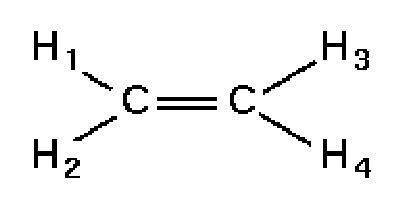
\includegraphics[angle=0,width=3cm,keepaspectratio]{immagini/etene/etene.eps}
\end{center}
\end{figure}
e assumendo che con angolo diedro A-B-C-D si intende l'angolo formato dai
piani definiti da A,B,C e B,C,D, la rotazione attorno al doppio legame 
viene studiata vincolando le torsioni H$_1$-C-C-H$_3$ e H$_2$-C-C-H$_4$, 
modificandone il valore da $0^{\circ}$ a $180^{\circ}$, ed eseguendo
l'ottimizzazione geometrica sui restanti gradi di libert\`a. Ne risulta
la superficie di potenziale, mostrata in figura \ref{fig:etene_3d}.

\begin{figure}[ht]
\begin{center}
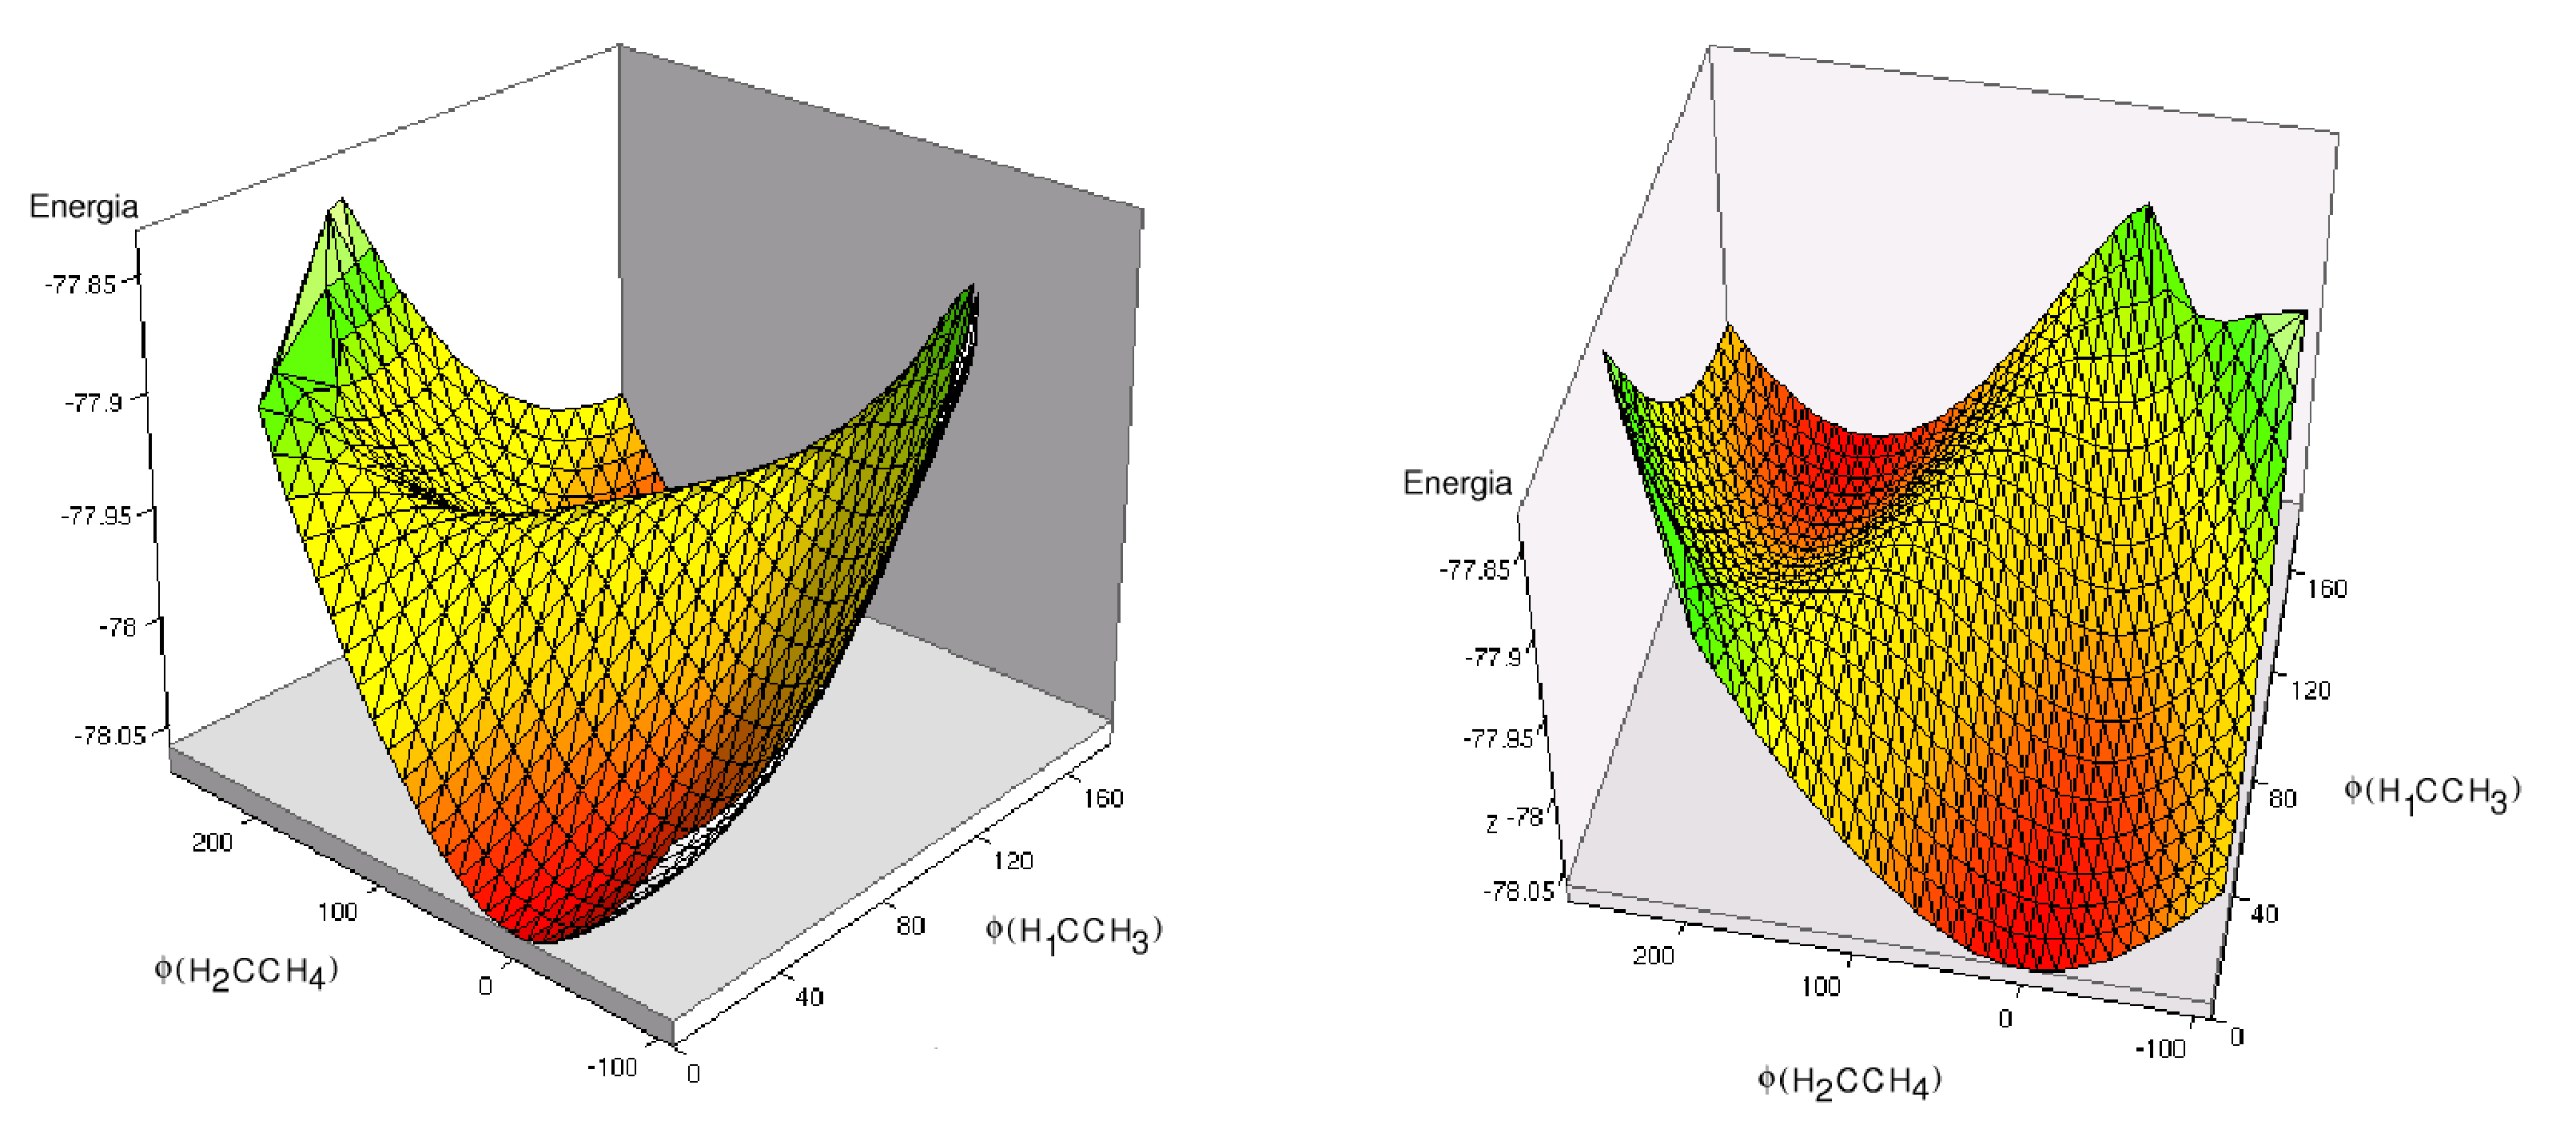
\includegraphics[angle=0,width=12cm,keepaspectratio]{immagini/etene/3d.eps}
\caption{\small Etilene - superfici di potenziale}
\label{fig:etene_3d}
\end{center}
\end{figure}

\`E possibile notare come tale superficie presenti due valli parallele,
ciascuna delle quali degenera in una spalla quando l'energia del minimo
diviene eccessivamente elevata. Una sezione della superficie a 
H$_1$-C-C-H$_3$ pari a 90$^{\circ}$ mostra un doppio minimo, con energie comparabili. 
\begin{figure}[ht]
\begin{center}
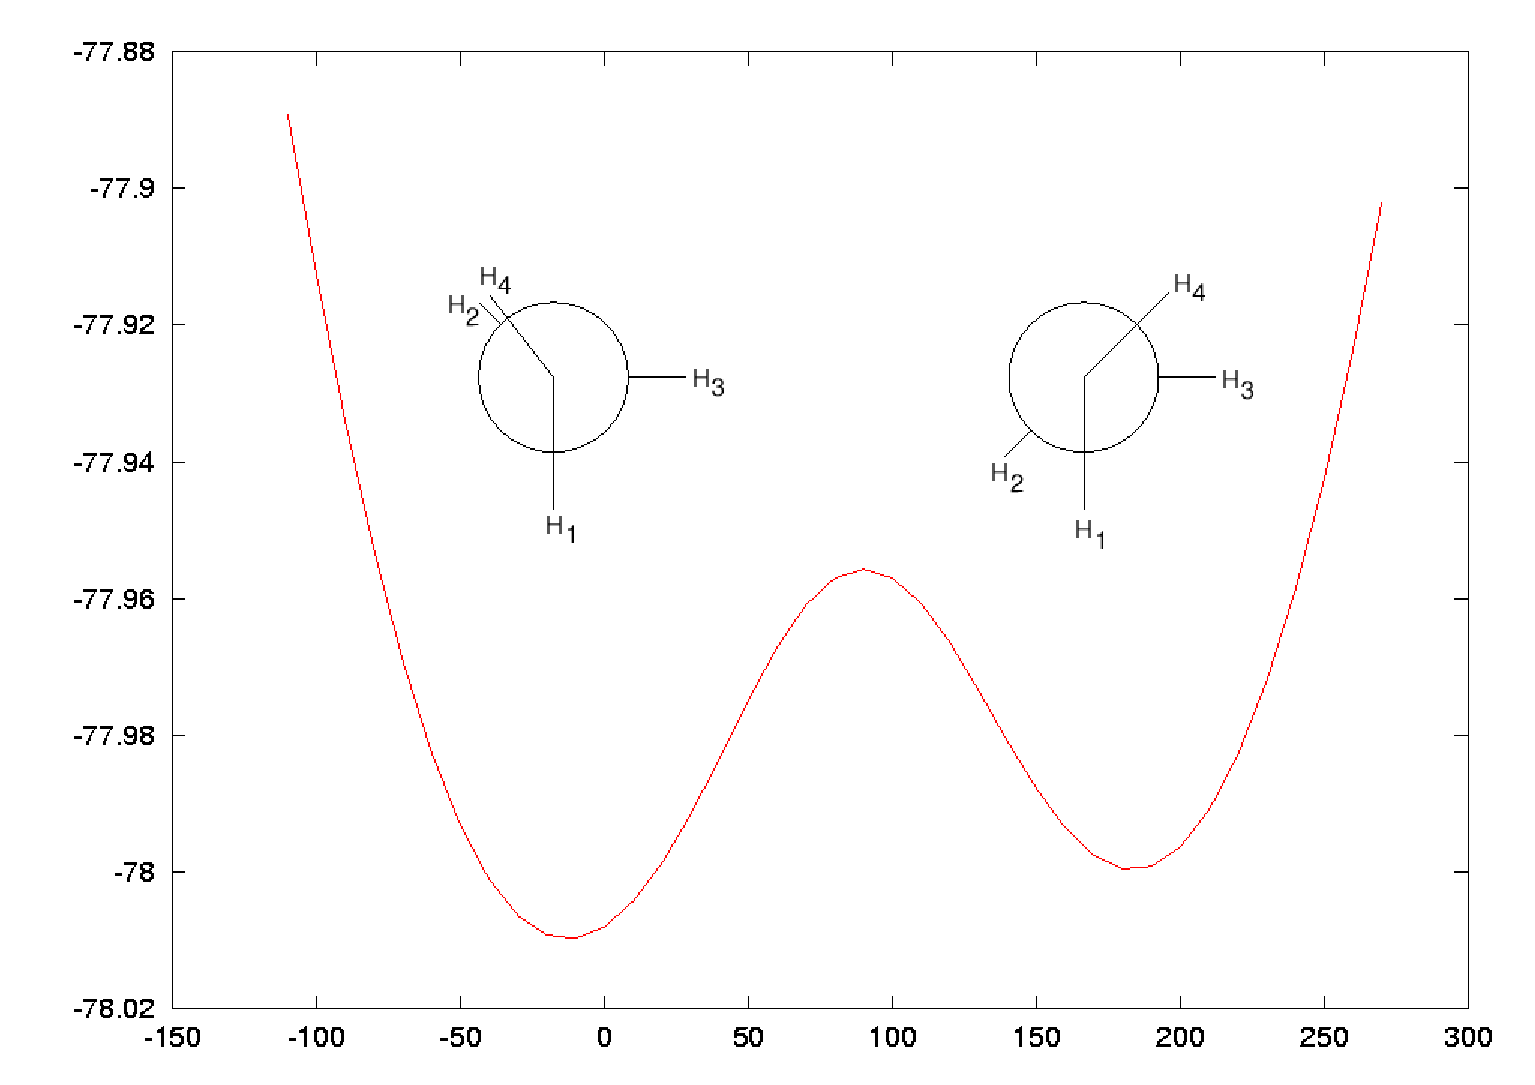
\includegraphics[angle=0,width=10cm,keepaspectratio]{immagini/etene/c090.eps}
\caption{\small Etilene - curva di potenziale rispetto all'angolo diedro
H$_2$-C-C-H$_4$. L'angolo diedro H$_1$-C-C-H$_3$ \`e fissato a 90$^{\circ}$}
\label{fig:etene_c090}
\end{center}
\end{figure}

Entrambi i minimi descrivono una possibile organizzazione spaziale a minima
energia della molecola in queste condizioni: la differenza, come \`e 
\begin{wrapfigure}{l}{6cm}
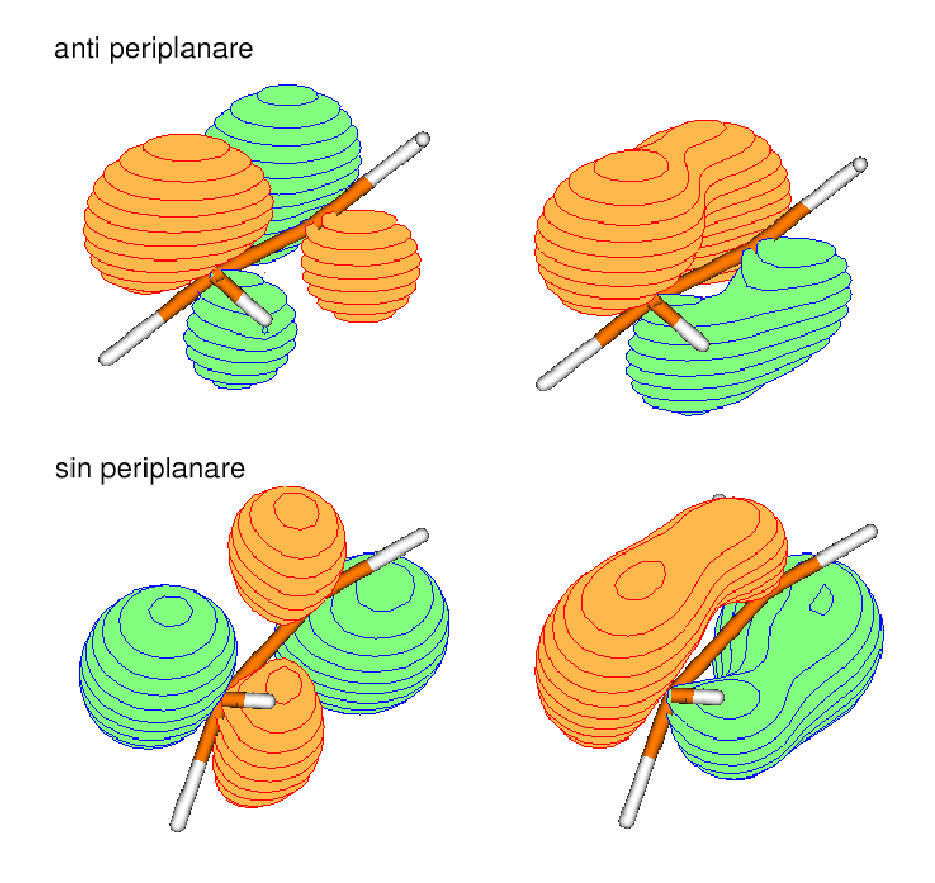
\includegraphics[angle=0,width=55mm,keepaspectratio]{immagini/etene/orbitali_c090.eps}
\caption{\small Etilene - orbitali dello spazio attivo (diedro H$_1$-C-C-H$_3$ a 90$^{\circ}$)}
\label{fig:etene_orbitali_c090}
\end{wrapfigure}
possibile notare dalla figura \ref{fig:etene_c090}, deriva dal diverso
posizionamento degli idrogeni H$_2$ e H$_4$, che assecondano i vincoli e la
necessit\`a di piramidalizzazione disponendosi in due diverse configurazioni
coplanari, una sin-periplanare, l'altra anti-periplanare. Il minimo
sin-periplanare possiede energia minore, anche a livello puramente nucleare,
sebbene presenti due atomi di idrogeno in posizione eclissata.
Gli orbitali attivi in queste due condizioni sono rappresentati in
figura \ref{fig:etene_orbitali_c090}.
La barriera di potenziale necessaria ad interconvertire, lungo questo grado
di libert\`a, la forma sin in forma anti \`e approssimativamente 1.45 eV, e passa per un
intermedio planare in cui gli orbitali $p$ degli atomi di carbonio sono
ortogonali.
L'utilizzo dell'etilene come esempio dimostrativo della superficie non
consente la distinzione tra isomero cis ed isomero trans, distinzione
che sar\`a apprezzabile nell'esatriene.

